\documentclass{article}

\usepackage{mathtools}
\usepackage[margin=1.5in]{geometry}
\usepackage{float}
\usepackage{verbatim}
\usepackage{graphicx}
\usepackage{amsthm}
\usepackage{xfrac}
\usepackage{tikz} % oh ho...
%\usepackage{svg} % I gave up...

\restylefloat{table}

\author{Guillaume Labranche (260585371)}
\title{COMP 531 -- Advanced Theory of Computation\\Assignment \#2}
\date{due on 15 February 2016}

\newcommand{\R}{\mathbb{R}}
\newcommand{\F}{\mathbb{F}}
%\newcommand{-->}{\rightarrow} %does not work :(
\newtheorem{theorem}{Theorem}
\newtheorem{corollary}{Corollary}
\newtheorem{lemma}{Lemma}
\newtheorem{proposition}{Proposition}

\newenvironment{definition}[1][Definition.]{\begin{trivlist}
\item[\hskip \labelsep {\bfseries #1}]}{\end{trivlist}}

\begin{document}

\pagenumbering{gobble}
\maketitle

\section{Logspace closed under composition}

Here we assume that by log-space computable functions, we mean functions which can be computed by a log-space transducer, that is a TM with a read-only input tape, a log-space bounded work tape and a write-only output tape.

\begin{theorem}If both $f$ and $g$ are computable in logarithmic space, $f \circ g$ is also computable in logarithmic space.
\end{theorem}
\begin{proof} In the trivial solution, for any input $x$ to $f \circ\ g$, we first compute $g(x)$ and then run $f$ on $g(x)$'s output tape. Let $n=|x|$. While $g(x)$ requires logarithmic work space, its output may be polynomial (by lemma \ref{lemma:logspace_polynomial}). Let $n' = |g(x)| = O(n^k)$. Then $f(g(x))$ requires $O(\log(n^k)) = O(k \log n) = O(\log n)$ work space. Although individually $f$ and $g$ only require logarithmic space, storing $g(x)$ requires polynomial space. Therefore we devise a trick that enables us to compute $f(g(x))$ without storing $g(x)$.

We modify the transducer $F$ for computing $f$ as follows. Whenever $F$ reads the $i$th symbol of its input tape (which contains $g(x)$), it runs the transducer $G$ for $g$ on $x$ until the $i$th symbol is outputted (transducers have a write-only output tape). This can be done using two counters of size $O(\log(n^k))=O(\log n)$ each, one for storing the position on $F$'s input tape and one for keeping track of the number of symbols outputted by $G$. As we can see, $f \circ g$ is still computable in logarithmic space because we do not store $g(x)$, only one character at a time and two counters of logarithmic size.
\end{proof}

\begin{lemma}\label{lemma:logspace_polynomial}
The output of a log-space computable function $f$ is polynomial in the size of its input.
\end{lemma}
\begin{proof}
Assuming that the log-space transducer outputs 1 symbol at every step of its runtime (without loss of generality), by first obtaining a bound on its runtime we can then bound the size of its output. The number of possible configurations is $|Q| \cdot (c \cdot \log_2 n) \cdot 2^{c \cdot \log_2 n} = O(2^{c \cdot \log_2 n}) = O(n^c)$. Since we know that $f$ is computable, the log-space transducer will terminate in finite time. The maximum number of configurations it can be in without looping forever is polynomial, and therefore so is the maximum number of symbols it can write to its output tape.
\end{proof}

\newpage
\section{Cycle searching principle}

The key intuition here is to realize that the son's future \textbf{and} past behaviour is entirely determined by the current edge (and direction) that he is following. With this insight, we can show that he cannot enter a cycle and get stuck in it unless he was spawned in it by his father. This is then used to show that the son always returns to his initial spawn vertex in finite time. Termination follows from that naturally while correctness requires some more detailed case analysis.

\begin{lemma}\label{lemma:deter}
Let $(v,w)\in E$, $(u_1,v,w)$ and $(u_2,v,w)$ be two paths followed by the son at some point during the execution of the algorithm. We claim that $u_1=u_2$.
\end{lemma}
\begin{proof}
Let $(v,w)$ be $v$'s $i$th edge. Therefore by the algorithm behaviour, $(u_1,v)$ is $v$'s $(i-1)$th edge. But $(u_2,v)$ is also $v$'s $(i-1)$th edge. Therefore it must be that $u_1=u_2$.
\end{proof}

\begin{definition}
We define a \textbf{son-loop} as a sequence of vertices $(u,v,\dotsc,u,v)$ such that when the son goes from $u$ to $v$, he will always come back to $u$ then $v$ and would loop forever unless his father is somewhere in the loop to stop him.\end{definition}

\begin{lemma}\label{lemma:sunloop}
If the son is outside of any son-loop, he cannot enter one.
\end{lemma}
\begin{proof}
Consider a son-loop $L=(u,v,\dotsc,w,u)$. Assume the son enters the cycle through vertex $u$ and then follows $(u,v)$ without loss of generality. By lemma \ref{lemma:deter}, the son was on vertex $w$ before entering the son-loop, which leads to a contradiction since $w \in L$. Either he was in the sun-loop all along, or he did not enter it.
\end{proof}

\begin{lemma}\label{lemma:finite}
After being brought to vertex $u$ by his father, the son always returns to $u$ in finite time.
\end{lemma}
\begin{proof} (by contradiction).

Assume the son never returns to $u$. By the pigeonhole principle, since there are only $2|E|$ possible ways to follow any edge ($|E|$ edges and 2 directions), the son must be following the same edge $v$ in the same direction at least twice. By the deterministic nature of the algorithm, he will then follow the exact same path when leaving $v$ and end up in a sun-loop. In the case that he was spawned in that sun-loop (on vertex $u$), since any sun-loop must have finite length, the son will return to $u$, which contradicts our assumption. It must then be the case that the son was spawned outside of the sun-loop and later entered it. But lemma \ref{lemma:sunloop} shows that this is not possible. Therefore our assumption cannot be true and the son will return to $u$.
\end{proof}

\begin{theorem}This algorithm terminates in finite time.\end{theorem}
\begin{proof} $\forall v\in V, \forall (v,u)\in E$, the son follows $(v,u)$ and by lemma \ref{lemma:finite} comes back to $v$ in finite time. Since $|V|$ and $|E|$ are both finite, the algorithm terminates in finite time.

\begin{comment}
$\forall v\in V, \forall (v,u)\in E$, the son follows $(v,u)$ and comes back to $v$ through $(u,v)$. Since $V$ and $E$ are finite, the only way for the algorithm to not be able to evaluate the condition is if the son does not ever come back to $v$. By the pigeonhole principle, since $V$ is finite the son must follow one edge more than once. The son's behaviour at a particular vertex $v$ is solely dependant on the previous visited vertex and the edges of $v$. Since $G$ does not change during the algorithm's runtime, visiting the same edge in the same direction twice will lead to the exact same behaviour and the son will be stuck in a loop. We will show that such a loop cannot exist.

Let $s\in V$ be a vertex where the son was taken to by his father. Assume that there is a loop in the path taken by the son and let $(v,w)\in E$ be the first edge that he visits twice in his path $P=(s,\dotsc,u_1,v,w,\dotsc,u_2,v,w,\dotsc)$. By lemma \ref{lemma:deter}, $u_1=u_2$ and $(u_1,v)=(u_2,v)$ is a repeated edge visited before $(u,v)$, which contradicts our assumption. Therefore there cannot be such a loop in his path and he will eventually return to $s$.
%When entering a vertex $u$ of fanout $k$, the son will follow edges $(i+1,i+1,$
%When following the edge $(v,u)$, the son follows all other edges of $u$ before coming back through $(v,u)$. 
%The son traverses the graph following the ``cycle searching principle'', starting at every vertex once. Therefore I will show that this principle terminates 
\end{comment}
\end{proof}

\begin{theorem}This algorithm detects a cycle $\iff$ there is a cycle.\end{theorem}
\begin{proof}
($\implies$) Consider the only way that the algorithm detects a cycle: When the son is placed at a vertex $v$, leaves through an edge $(v,u)$ and comes back to $v$ through a different edge $(w,v)$ where $u\not=w$. In this case, there is a path from $v$ to $u$, from $u$ to $w$ and from $w$ to $v$. This forms a cycle.

($\Longleftarrow$) Suppose there is a cycle $C$ containing the edge $(u,v)$. Then at some point the father will bring the son to $u$ and send it along the edge of $v$. By lemma \ref{lemma:finite}, the son will always return to $u$. Now consider two cases:
\begin{itemize}
\item If the son does not come back through $(u,v)$, the cycle is detected.
\item If the son does come back through $(u,v)$, then there must be a vertex $w \in C$ such that the son did not enter the successor of $w$ in $C$ (in other words he must have left $C$ at some vertex $w$). Since $w$ is connected to its successor, its predecessor and some other vertices, its fanout is at least 3. Assume that the predecessor and successors of $w$ are accessible through the $i$th and $j$th edges of $w$ respectively. Then the son must leave $C$ at $w$ through the $k$th edge of $w$ where $i<k<j$ otherwise he would have reached the successor of $w$ first and by definition it does not happen. Now consider 3 subcases:
\begin{itemize}
\item If the son leaves the cycle from $w$ and comes back to $w$ through a different edge, then when the father brings him to $w$ he will detect a cycle.
\item If the son comes back to $w$ through the same edge, then he will eventually reach the vertex following $w$ in $C$. But that contradicts our definition of $w$ which is supposedly the furthest vertex reached in $C$. Therefore this case is not possible. %That will bring him back to $u$ from the other end of $C$ and the cycle will be detected.
\item If the son does not come back to $w$, then he must eventually re-enter $C$ through one of the vertices he already visited. Let's call that vertex $z$. When later in the algorithm the father brings the son to $z$ and sends him to the successor of $z$ in $C$ called $z'$, due to the deterministic nature of the algorithm, the son will follow the same path as just described and not return to $z$ through the same edge (since we defined $z$ as the vertex where the son re-enters $C$). At that time, the father will notice the different return edge and detect a cycle.
\end{itemize}
\end{itemize}

\begin{figure}[!h]
\centering
\begin{tikzpicture}
\def \n {7}
\def \radius {2cm}
\def \margin {10} % margin in angles, depends on the radius

\def \s {5}
  \node[draw, circle] at ({360/\n * (\s - 1)}:\radius) {$u$};
\def \s {4}
  \node[draw, circle] at ({360/\n * (\s - 1)}:\radius) {$v$};
\def \s {1}
  \node[draw, circle] at ({360/\n * (\s - 1)}:\radius) {$w$};


\def \s {1}
  \draw[-, >=latex] ({360/\n * (\s - 1)}:\radius + \margin)
    -- ({360/\n * (\s - 1)}:\radius * 1.75);

\def \s {2}
  \draw[dashed,<-, >=latex] ({360/\n * (\s - 1)+\margin}:\radius)
    arc ({360/\n * (\s - 1)+\margin}:{360/\n * (\s)-\margin}:\radius);
\def \s {6}
  \draw[dashed,<-, >=latex] ({360/\n * (\s - 1)+\margin}:\radius)
    arc ({360/\n * (\s - 1)+\margin}:{360/\n * (\s)-\margin}:\radius);

\foreach \s in {2,3,6,7}
{
  \node[draw, circle] at ({360/\n * (\s - 1)}:\radius) {\text{}};
}
\foreach \s in {1,3,4,5,7}
{
  \draw[<-, >=latex] ({360/\n * (\s - 1)+\margin}:\radius)
    arc ({360/\n * (\s - 1)+\margin}:{360/\n * (\s)-\margin}:\radius);
}
\end{tikzpicture}
\caption{Diagram illustrating a cycle $C$ in $G$}
\end{figure}

\begin{comment}
($\Longleftarrow$) When following edge $(v,u)$, the son following the ``cycle searching principle'' always visits all the neighbours of $u$ in sequential order before going back through $(u,v)$. Therefore if the vertex $v$ is the root of a tree (acyclic graph) the son will perform a tree traversal, coming back along an edge only if the subtree has been been entirely visited. In the case that there is a cycle containing $v$, $u$ and $w$ where $(v,u),(v,w)\in E$, the son will eventually be brought to $v$ by his father. The son will leave $v$ through the edge $(v,u)$ and eventually reach $w$. At that point he will re-enter $v$ and the cycle will be detected.
\end{comment}
\end{proof}

The algorithm only needs to store a constant amount of vertex indices:
\begin{itemize}
\item which vertex the father is visiting
\item which vertex the son visits initially
\item which vertex the son last visited while traversing the graph
\end{itemize}

Therefore the space complexity is $O(\log |V|)$.
Also worth noting is that this algorithm works for both connected and disconnected graphs.

\section{Boolean symmetric functions $\rightarrow$ MAJ $\circ$ MAJ}

First we note that the description of a symmetric boolean function $f:\{0,1\}^n\rightarrow \{0,1\}$ is basically a mapping $m:\{0,1,\dotsc,n\}\rightarrow \{0,1\}$.

Next, we introduce a new type of gate MAJ$_{\geq i}$ constructed from a single MAJ gate that returns 1 when $i$ or more of its $n$ input wires are 1, and 0 otherwise. To construct it, we feed all $n$ inputs into a MAJ gate. We also add $i$ 0-constant inputs and $n-i+1$ 1-constant inputs for a total of $2n+1$ inputs. Therefore the MAJ gate will output 1 when:
\begin{align*}
\#_1 &> \frac{2n+1}{2} \\
\#_1 &> n + \sfrac{1}{2} \\
\#_1 &\geq n + 1 \\
\#_1 &\geq i + (n-i+1 \text{ 1-constants})
\end{align*}
Therefore when ignoring the constants, our MAJ$_{\geq i}$ will return 1 when $i$ or more of its $n$ inputs are 1. The following diagram illustrates the strategy visually:

\includegraphics{q3_maj_geq.pdf}

\begin{comment}
Its construction is divided in two cases:
\begin{itemize}
\item $i \geq \sfrac{n}{2}$: We simply feed all $n$ inputs into a MAJ gate and add 0-constant inputs until the gate has $2i-1$ inputs. The gate will output 1 when: 
\begin{align*}
\#_1 &> \frac{2i-1}{2} \\
\#_1 &\geq i
\end{align*}
where $\#_1$ denotes the number of non-constant inputs (i.e. the one that matter) into the gate with value 1.
\item $i < \sfrac{n}{2}$: 
\end{itemize}
\end{comment}

We also introduce a similar gate MAJ$_{\leq i}$ that returns 1 if $i$ or less inputs are 1 and 0 otherwise. Its construction is very similar to MAJ$_{\geq i}$ but with negated inputs. Checking whether there are at most $i$ 1s is equivalent to checking whether there are more than $n-i$ 0s. Thus we negate all $n$ inputs and feed them into a MAJ gate. We then add $n-i$ 0-constant inputs and $i+1$ 1-constant inputs so that the MAJ gate has fanin $2n+1$. Therefore the MAJ gate will output 1 when:
\begin{align*}
\#_1 &> \frac{2n+1}{2} \\
\#_1 &> n + \sfrac{1}{2} \\
\#_1 &> n \\
\#_0 &\leq n \\ 
\#_0 &\leq i + (n-i \text{ 0-constants})
\end{align*}
Since we negated the $n$ inputs, this is equivalent to checking that $$\#_1(\text{original input}) \leq i$$

We then introduce a new type of gate EQ$_i:\{0,1\}^n\rightarrow\{0,1\}\times\{0,1\}$ composed of a MAJ$_{\geq i}$ and a MAJ$_{\leq i}$. On input $w$, it will output $(1,1)$ if $\#_1(w)=i$, and $(1,0)$ (or $(0,1)$) if $\#_1(w)\not=i$.

Now to construct a circuit to compute $f$, for all $i$ such that $f(i)=1$, add an EQ$_i$ gate with the same inputs as $f$ at level 1.  At level 2, add a single MAJ gate taking all our level 1 gates as input.

In order to show that this indeed computes $f$, let's perform a case analysis on $f(j)$ for all $0\leq j \leq n$:
\begin{itemize}
\item $f(j)=1$: This will make all the EQ$_{i\not=j}$ return $(1,0)$ or $(0,1)$ except the gate EQ$_{i=j}$ which will return $(1,1)$. There will be more 1s than 0s feeding into the level 2 MAJ gate and the circuit will output 1.

\item $f(j)=0$: This will result in all EQ gates returning $(1,0)$ or $(0,1)$ since no EQ$_{i=j}$ gate has been added to the circuit. Therefore the number of 0s and 1s will be equal and the level 2 MAJ gate will output 0.

\end{itemize}

Note that this also creates a circuit of linear size, since $f(i)=1$ for at most $n$ values and that in each of those cases we add 2 MAJ gates. This completes the construction of a linear-size MAJ $\circ$ MAJ circuit computing a symmetric boolean function. 

\newpage
\section{Polysize circuits $\rightarrow$ NC\textsuperscript{1}}

In order to show that the boolean function induced from a polysize tree-shaped circuit is actually in $NC^1$, we describe a transformation of such circuits to equivalent polysize circuits of logarithmic depth.

Let $F(x_1,\dotsc,x_n)$ be the boolean formula induced from a circuit $C_n \in C$ with root node $u$ and size $s=O(n^k)$. Starting a $u$, find a subtree of size $t$ where $\frac{1}{3}s\leq t \leq \frac{2}{3}s$ using the strategy described in lemma \ref{lemma:subtree} and call its root $v$. Let $F'(x_1,\dotsc,x_n)$ be the boolean formula represented by this subcircuit. See figure \ref{fig:original} for an illustration.

Now take the subtree rooted at $v$ out of our main circuit and replace it with a variable called $z$. We now have two trees rooted at $u$ and $v$, each of size at most $\frac{2}{3}s$. Let $\hat{F}(x_1,\dotsc,x_n,z)$ be the formula represented by the circuit rooted at $u$ after removing the $u$ subtree. 

We now construct a new circuit equivalent to our original as shown in figure \ref{fig:transformed}. In order for our new circuit to return 1, we join two cases by an $\lor$ gate.
\begin{itemize}
\item In the first case we assume the circuit rooted at $v$ returns 1. In order to not modify the output of the circuit, we join the following two conditions by an $\land$ gate:
\begin{itemize}
\item Our original circuit must return 1 when $z=1$.
\item The subcircuit at $v$ must also return 1 since we set $z=1$.
\end{itemize}
\item The second case is when the subcircuit returns 0. We join the following two conditions by an $\land$ gate:
\begin{itemize}
\item Our original circuit must return 1 when $z=0$.
\item The subcircuit at $v$ must return 0 since we set $z=0$. In order to do that, we first negate the boolean formula: $\neg F'(x_1,\dotsc,x_n)$. We then use De Morgan's laws to push the negation all the way down to the inputs and negate the ones that are negated in the formula. We therefore do not need to add extra gates.
\end{itemize}
\end{itemize}

The result of this transformation is shown in figure \ref{fig:transformed}. Once this is done, we recursively apply this transformation on all the subtrees rooted at level 3 nodes of our new circuit. The recursion stops once we reach subtrees of size 1.

\begin{figure}[!h]
\centering
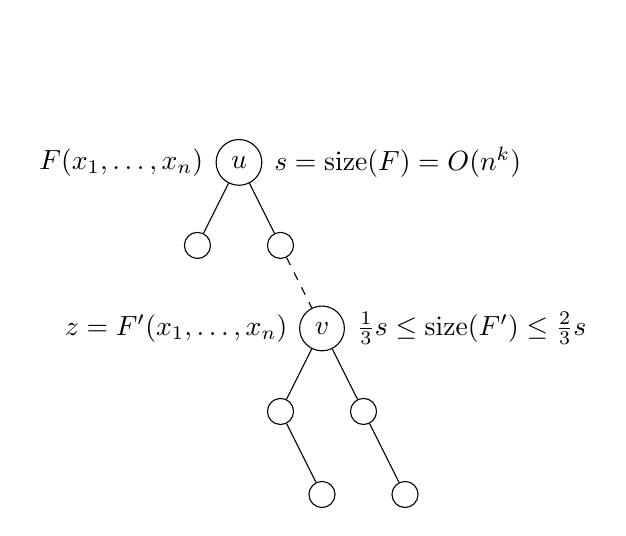
\begin{tikzpicture}[sibling distance=3em, level distance=3em,
  every node/.style = {shape=circle, rounded corners,
    draw, align=center}]
  \node[label={left:$F(x_1,\dotsc,x_n)$},label={right:$s=\text{size}(F)=O(n^k)$}] {$u$}
    child { node {} }
    child { node {}
      child[missing]
      child[dashed] { node[solid,label={left:$z=F'(x_1,\dotsc,x_n)$},label={right:$\frac{1}{3}s\leq\text{size}(F') \leq \frac{2}{3}s$}] {$v$} 
        child[solid] { node {} 
          child[missing]
          child { node {}}}
        child[solid] { node {}
          child[missing]
          child { node {}}}
      } };
\end{tikzpicture}
\caption{$C_n$ before the transformation}
\label{fig:original}
\end{figure}

\begin{figure}[!h]
\centering
\begin{tikzpicture}[level distance=3em,
  level 1/.style={sibling distance=18em},
  level 2/.style={sibling distance=9em},
  every node/.style = {shape=circle, rounded corners,
    draw, align=center}]
  \node[label={left:$F(x_1,\dotsc,x_n)$},label={right:$s=\text{size}(F)=O(n^k)$}] {$\lor$}
    child { node {$\land$}
      child { node[label={[label distance=-3em]below:$\hat{F}(x_1,\dotsc,x_n,1)$}] {}}
      child { node[label={[label distance=-3em]below:$F'(x_1,\dotsc,x_n)$}] {}}}
    child { node {$\land$}
      child { node[label={[label distance=-3em]below:$\hat{F}(x_1,\dotsc,x_n,0)$}] {}}
      child { node[label={[label distance=-3em]below:$\neg F'(x_1,\dotsc,x_n)$}] {}}};
\end{tikzpicture}
\caption{$C_n$ after one recursion step}
\label{fig:transformed}
\end{figure}

In order to show that this indeed creates a tree of depth $O(\log n)$, realize that one recursion step only adds a constant (2) depth to the newly created tree so far. Also note that the recursion is done on subtrees that are at most $\sfrac{2}{3}$ the size of the original tree. Therefore in the worst case, we have $\log_{\sfrac{3}{2}}(s)=O(\log n^k)=O(k\log(n))$. Therefore the depth of our final tree has depth logarithmic in the number of inputs.

In order for the transformed circuit to be in $NC^1$ we must also show that its size is polynomial. At every step of the recursion, we add a constant amount of gates and we also duplicate the subtrees without altering their number of gates. We therefore double the amount of gates at each step. Since there are $O(\log n)$ steps, we multiply the number of gates by a factor of $2^{\log n}=n$. Therefore this only increases the degree of the polynomial by 1 which is still a polynomial amount of gates in terms of the number of inputs $n$.

\begin{lemma}\label{lemma:subtree}
Given a tree of size $s$ with root node $u$, there is a node $v$ whose subtree is of size $t$ where $\frac{1}{3}s\leq t \leq \frac{2}{3}s$
\end{lemma}
\begin{proof}
If either the immediate left or right child of $u$ is a subtree size $t$, then we have found $v$. Otherwise, recurse on the child whose subtree is bigger. Because each recursion step reduces the size of the tree by at least one, we are guaranteed to find such $v$.
\end{proof}

% into constant-height to reduce their heights by a constant factor. We then apply the same .

\section{$w$-parity}

Left blank due to lack of time.
%Sadly I have a MATH-340 assignment worth as much as question 5 due the next day at 8:30am. I do not have enough time to complete this question.

\end{document}
